\documentclass[numbering=fraction,aspectratio=169]{beamer}


% -------------------------------
% Packages
% -------------------------------
\usepackage{fontspec}
  \setmainfont{Latin Modern Roman}
  \newfontfamily\emoji{NotoColorEmoji}[Renderer=HarfBuzz]
\usepackage{polyglossia}
  \setdefaultlanguage[variant=brazilian]{portuguese}
\usepackage{hyperref}
\usepackage{xspace}
\usepackage{graphicx}
\usepackage{multicol}
\usepackage{makecell}
\usepackage{circledsteps}
\usepackage{tikz}
\usetikzlibrary{arrows.meta, positioning}


% -------------------------------
% Theme and Styling
% -------------------------------
\usetheme[progressbar=frametitle]{metropolis}

% Colors
\definecolor{impatechpink}{RGB}{254,137,239}
\definecolor{impatechorange}{RGB}{254,196,84}
\definecolor{impatechgreen}{RGB}{189,255,139}

% Title page logo
\titlegraphic{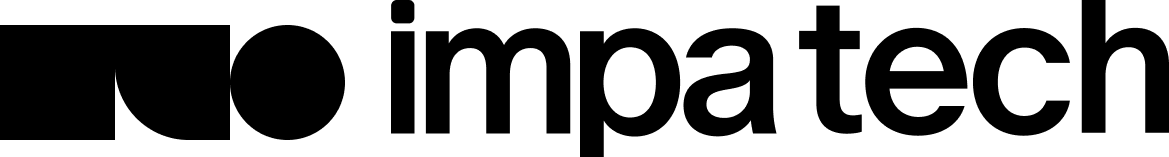
\includegraphics[width=3cm]{img/impatech-logo}}

% Color theme and font adjustments
\setbeamercolor{frametitle}{fg=black, bg=impatechorange}
\setbeamercolor{title separator}{fg=impatechorange}

\setbeamercolor{block title alerted}{fg=black, bg=impatechpink}
\setbeamercolor{block body alerted}{fg=black, bg=impatechpink!30}
\setbeamercolor{alerted text}{fg=impatechpink}
\setbeamerfont{alerted text}{series=\bfseries}

\setbeamercolor{block title example}{fg=black, bg=impatechgreen}
\setbeamercolor{block body example}{fg=black, bg=impatechgreen!30}
\setbeamercolor{footline}{fg=gray}
\setbeamercolor{progress bar}{fg=black}

% Footer
\setbeamertemplate{frame footer}{\insertshortinstitute\ | HU31 | \insertshortauthor\ | 2026.1 }


% -------------------------------
% Custom commands
% -------------------------------
\newcommand\IMPATech{\textsc{impa}\,Tech\xspace}
\newcommand{\gap}{\rule{1cm}{0.4pt}\ }
\newcommand\ThumbsUp{{\emoji 👍}\ }
\newcommand\ThumbsDown{{\emoji 👎}\ }
\newcommand\WarningEmoji{{\emoji ⚠️}\ }
\newcommand{\Link}[2]{\href{#1}{\texttt{#2}}}
\newcommand{\FigureCaption}[1]{{\scriptsize #1}}

\pgfkeys{/csteps/fill color=black}
\pgfkeys{/csteps/inner color=impatechorange}
\newcommand{\CircledNumber}[1]{\Circled{\textbf{#1}}\xspace}


% -------------------------------
% Custom counter
% -------------------------------
% From https://tex.stackexchange.com/questions/55000/continuing-enumerate-counters-in-beamer
\newcounter{saveenumi}
\newcommand{\seti}{\setcounter{saveenumi}{\value{enumi}}}
\newcommand{\conti}{\setcounter{enumi}{\value{saveenumi}}}


% -------------------------------
% URLs
% -------------------------------
% \def \ExampleURL{https://example.com/}
\def \ProgramaURL{https://docs.google.com/spreadsheets/d/1GIyGNly4fYUiEZCE9rLsmmhvgb5aWTR_2kg0VaIVGIc/}
\def \TiktaalikURL{https://science.psu.edu/news/Stewart4-2024}


% -------------------------------
% Title page metadata
% -------------------------------
\title{Aula 15: as limitações do Falsificacionismo}
\author[Rafael Beraldo]{Rafael Luis Beraldo\\
  \texttt{<\href{mailto:rafael.beraldo@impatech.edu.br}{rafael.beraldo@impatech.edu.br}>}\\
  \textbf{HU31 – Epistemologia da Ciência}}
\institute{\IMPATech}
\date{21 de maio de 2026}


% -------------------------------
% Main document
% -------------------------------
\begin{document}
\frenchspacing

\begin{frame}[plain]{}
  \maketitle
\end{frame}



\section{De onde viemos e para onde vamos}

\begin{frame}{Na aula anterior…}
  \begin{itemize}
  \item Vimos como o \alert{grau de falsificabilidade} permite a comparação entre hipóteses e explica o progresso científico.
  \item Diferenciamos modificações teóricas produtivas das puramente \alert{\emph{ad hoc}}.
  \item Discutimos o papel da \alert{confirmação} no falsificacionismo.
  \end{itemize}
\end{frame}

\begin{frame}{Objetivos desta aula}
  \begin{itemize}
  \item Compreender as \alert{limitações do falsificacionismo} de Popper.
  \item Analisar como \alert{hipóteses auxiliares} e condições experimentais complexificam as situações de teste.
  \item Entender que a história mostra que teorias científicas frequentemente \alert{sobrevivem a aparentes refutações}.
  \end{itemize}
\end{frame}



\section{As rachaduras do Falsificacionismo}

\begin{frame}{O falsificacionismo ingênuo e o falsificacionismo sofisticado}
  \begin{itemize}
  \item<1-> Qual o \alert<1>{papel da refutação} (= falsificação) de uma hipótese para o falsificacionista?
  \item<2-> O que significa \alert<2>{“confirmar” uma hipótese} para o falsificacionista?
  \item<3-> Têm em comum: \alert<3>{aceitações são sempre tentativas}; apenas \alert<4>{refutações podem ser definitivas}.
  \end{itemize}
\end{frame}

\begin{frame}{Questões para discutir}
  \begin{itemize}
  \item<1-> Se a lógica da refutação exige uma \alert<2>{observação} para falsificar uma teoria, onde reside \alert<1-2>{a fraqueza} do falsificacionismo?
  \item<3-> Se todas as proposições de observação são falíveis, como podemos ter certeza de que um choque entre teoria e observação não é, na verdade, \alert<3>{um erro da observação e não da teoria}?
  \item<4-> Exemplo de Chalmers (2017, p.~91): Vênus não muda de tamanho aparente; a despeito disso, \alert<4>{a teoria copernicana não foi solapada}.
  \end{itemize}
\end{frame}



\section{A defesa inadequada de Popper}

\begin{frame}{Dois tipos de observação}
  Para Popper (Chalmers, 2017, p.~92), as observações dividem-se em:

  \begin{description}
  \item<2->[Observações privadas] Experiências perceptivas individuais.
  \item<3->[Observações públicas] Ou proposições de observação, \alert{motivadas pelas observações privadas e aceitáveis ou rejetáveis por observadores individuais}.
  \end{description}
\end{frame}

\begin{frame}{A defesa de Popper}
  \begin{quote}
    Any empirical \alert<1>{scientific statement} can be presented (by describing experimental arrangements, etc.) in such a way \pause that anyone who has learned the relevant technique can \alert<2>{test it}. \pause If, as a result, he \alert<3>{rejects the statement}, \pause then it will not satisfy us if he tells us all about his \alert<4>{feelings of doubt or about his feelings of conviction} as to his perceptions. \pause What he must do is to \alert<5>{formulate an assertion which contradicts our own}, and give us his \alert<5>{instructions for testing it}. \pause If he fails to do this we can only ask him to take another and perhaps a more \alert<6>{careful look at our experiment, and think again}.

    \raggedleft
    \small (Popper, 2002, p.~81)
  \end{quote}
\end{frame}



\section{Situações de teste são complexas}

\begin{frame}{Questões para discutir}
  \begin{columns}
    \column{0.6\textwidth}
    \begin{itemize}
    \item<1-> Uma teoria científica na vida real é uma \alert<1>{afirmação simples}, tal como “todos os cisnes são brancos”?
    \item<2-> Se uma previsão falha em um sistema teoria/condições iniciais/hipóteses auxiliares, a lógica nos permite \alert<2>{apontar com precisão qual dessas partes é a culpada}?
    \item<3-> Lembremos do exemplo do \emph{Tiktaalik}. O que aconteceria com a Evolução caso os cientistas \alert{não o tivessem encontrado}?
    \end{itemize}

    \column{0.4\textwidth}
    \uncover<3>{
      \begin{figure}
        \centering
        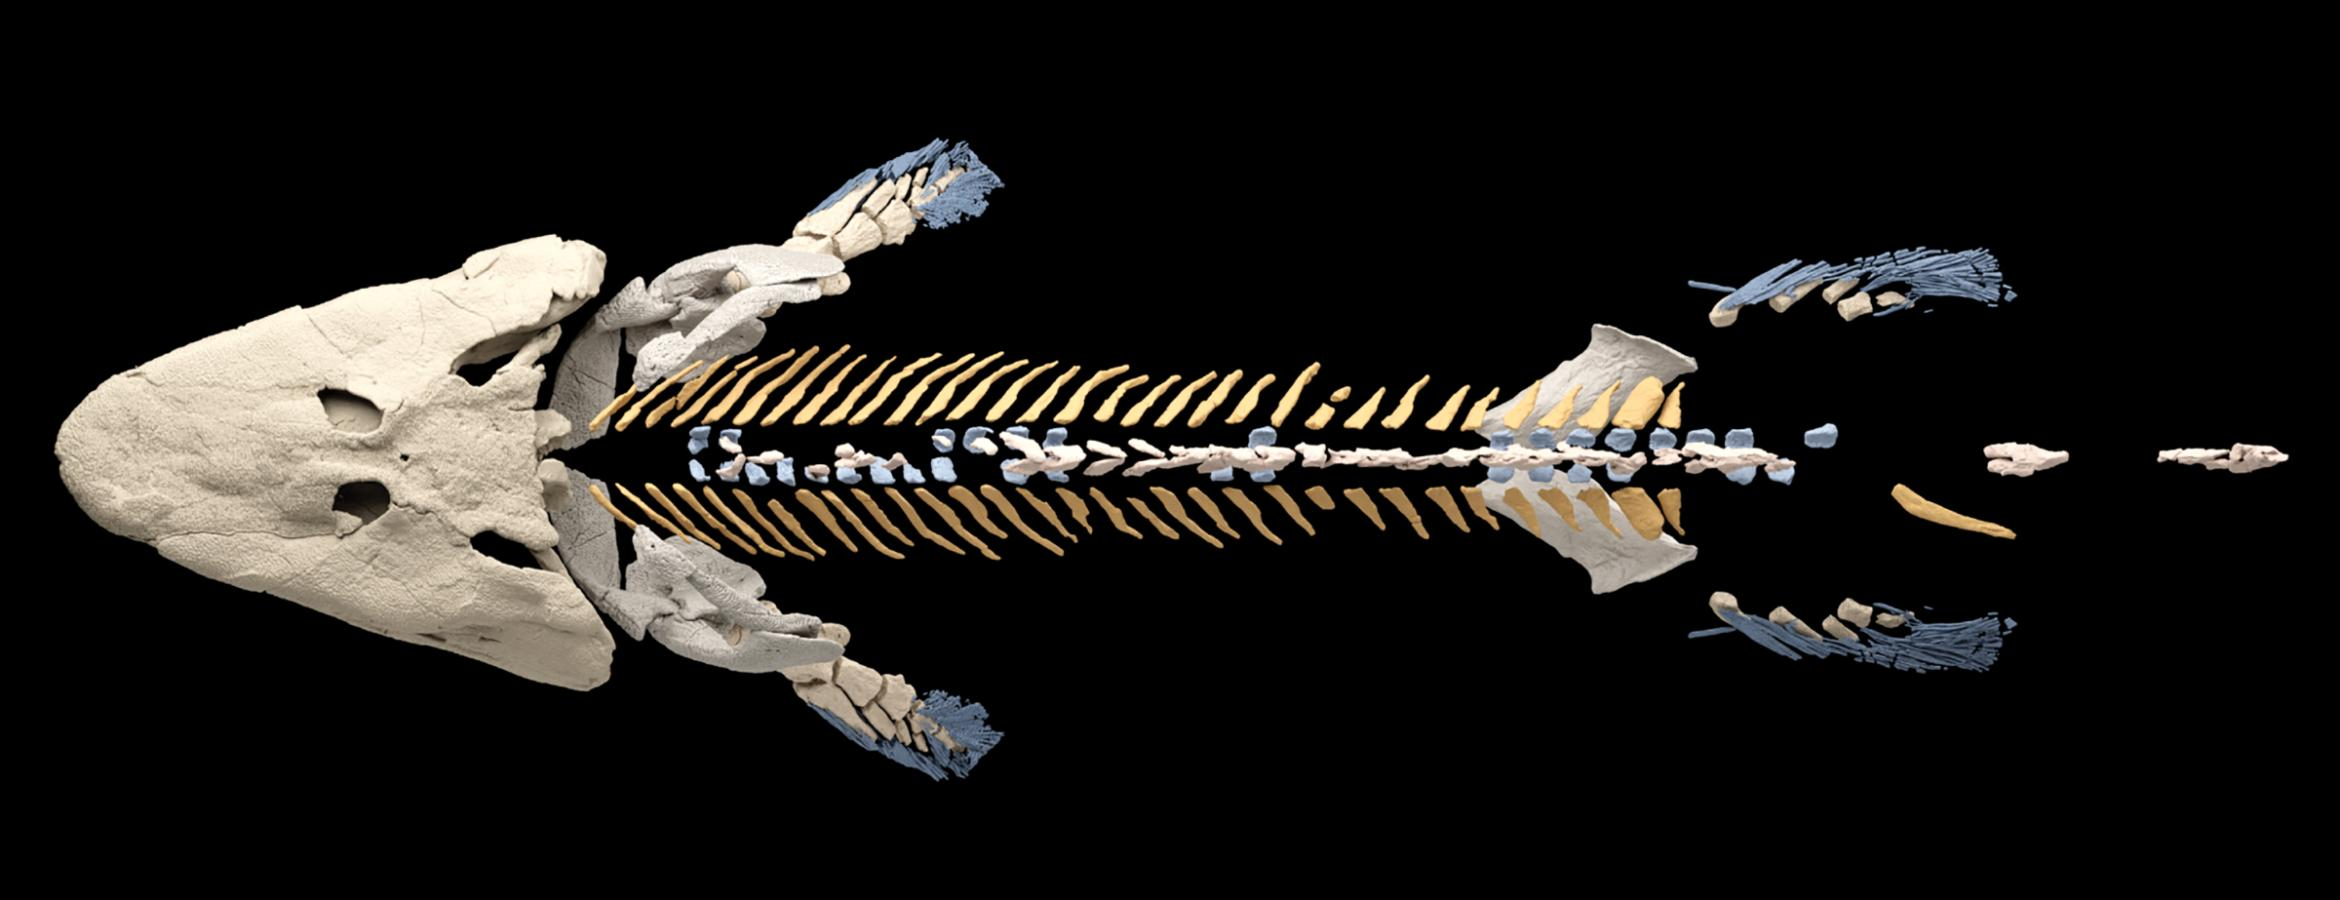
\includegraphics[width=\textwidth]{img/tiktaalik}
        \caption{Reconstrução do esqueleto do \emph{Tiktaalik}. Fonte: \href{\TiktaalikURL}{science.psu.edu}.}
      \end{figure}}
  \end{columns}
\end{frame}

\begin{frame}{Tycho Brahe vs. Copérnico}
   \begin{figure}
        \centering
        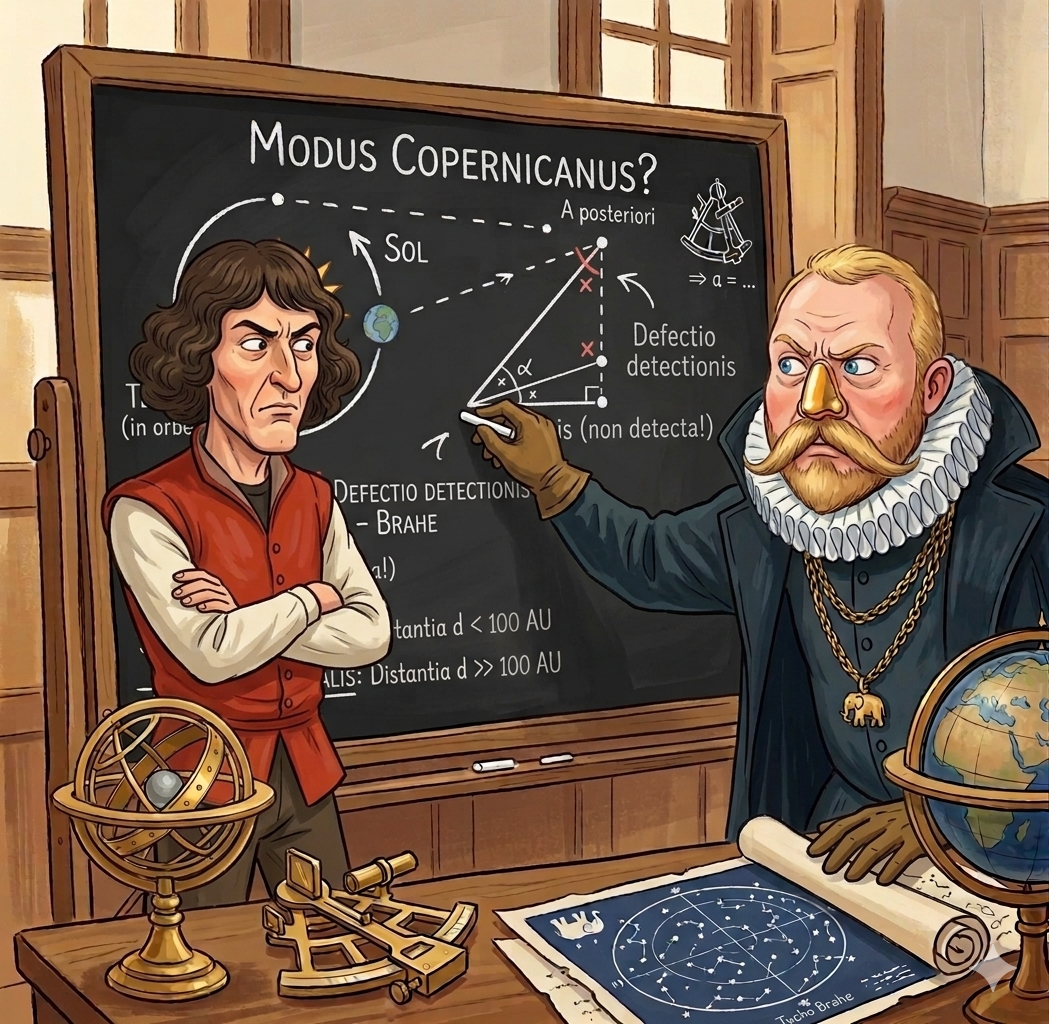
\includegraphics[height=5.5cm]{img/paralaxe}
        \caption{Imagem gerada pelo Gemini. Exemplo baseado em Chalmers (2017, p.~96)}
      \end{figure}
\end{frame}


\section{A história não apoia o falsificacionismo}

\begin{frame}{Questões para discutir}
  \begin{itemize}
  \item<1-> Se Newton tivesse \alert<1>{rejeitado sua teoria da gravitação logo na primeira dificuldade} com a órbita da Lua, o que teria acontecido com o desenvolvimento da física?
  \item<2-> Podemos dizer que uma teoria \alert<2>{nasce pronta}? \pause Ou ela precisa de \alert<3>{proteção e tempo} para se desenvolver, mesmo com aparentes refutações iniciais?
  \end{itemize}
\end{frame}

\begin{frame}{Contraexemplo histórico: Copérnico vs. Aristóteles Ptolomeu}
  \begin{itemize}
  \item<1-> A \alert<1>{física Aristotélica}
  \item<2-> A \alert<2>{proposta heliocêntrica} de Copérnico (1473--1543)
  \item<3-> Argumentos contra o movimento da Terra: \alert<3>{argumento da Torre}; constância do \alert<3>{tamanho aparente de Vênus}
  \item<4-> Vantagem copernicana: \alert<4>{simplicidade matemática}
  \item<5-> Galileu (1564--1642): \alert<5>{telescópio e nova mecânica}
  \item<6-> Kepler (1571--1630): \alert<6>{órbitas elípticas}; Newton (1643--1727): \alert<6>{síntese física}
  \end{itemize}
\end{frame}


\section{Hora do seminário!}



\section{Referências}

\begin{frame}[allowframebreaks]{Referências}
  \begin{thebibliography}{9}

  \bibitem{chalmers2017}
    CHALMERS, Alan F.
    \emph{O que é ciência, afinal?}
    São Paulo: Editora Brasiliense, 2017.

  \bibitem{popper2002}
    POPPER, Karl.
    \emph{The logic of scientific discovery}.
    London: Routledge, 2002.

  \end{thebibliography}
\end{frame}
\end{document}
